\documentclass{article}
\usepackage{graphicx} % For including diagrams

\title{RPC File Transfer Practical Work}
\author{Ha Tan Minh}
\date{}

\begin{document}

\maketitle

\section{Introduction}
The purpose of this practical is to implement a file transfer system using Remote Procedure Call (RPC). The system involves an XML-RPC server and client implemented in Python, where the server receives and stores files sent by the client.

\section{Protocol Design}
The file transfer protocol using RPC involves:
\begin{itemize}
    \item Exposing a remote procedure on the server for receiving files.
    \item The client encoding the file in Base64 and sending it to the server using the remote procedure.
    \item The server decoding the file and saving it.
\end{itemize}
\begin{figure}
    \centering
    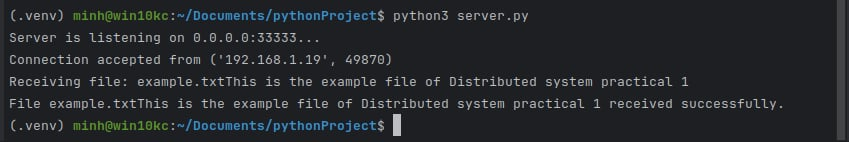
\includegraphics[width=1\linewidth]{a.png}
    \caption{Server}
    \label{fig:rpc-interaction}
\end{figure}

\section{System Interaction}

\begin{center}
Laptop 1 (Server)
\end{center}

\begin{figure}
    \centering
    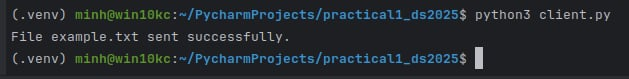
\includegraphics[width=1\linewidth]{b.png}
    \caption{Client}
    \label{fig:rpc-details}
\end{figure}

\begin{center}
Laptop 2 (Client)
\end{center}

\section{Implementation}
The implementation involves two Python scripts for the server and client.

\subsection{Server Code}
The server listens for incoming remote procedure calls and saves the file:
\begin{verbatim}
from xmlrpc.server import SimpleXMLRPCServer
import base64

def receive_file(filename, filedata):
    # Decode the file data
    file_bytes = base64.b64decode(filedata)
    with open(filename, 'wb') as file:
        file.write(file_bytes)
    print(f"File {filename} received successfully.")
    return f"File {filename} received successfully."

if __name__ == "__main__":
    server_ip = "0.0.0.0"
    server_port = 8000
    server = SimpleXMLRPCServer((server_ip, server_port))
    print(f"Server is listening on {server_ip}:{server_port}...")

    server.register_function(receive_file, "receive_file")
    server.serve_forever()
\end{verbatim}

\subsection{Client Code}
The client connects to the server and sends the file:
\begin{verbatim}
import xmlrpc.client
import base64

def send_file(server_url, filename):
    with open(filename, 'rb') as file:
        file_bytes = file.read()
        file_data = base64.b64encode(file_bytes).decode('utf-8')

    server = xmlrpc.client.ServerProxy(server_url)
    response = server.receive_file(filename, file_data)
    print(response)

if __name__ == "__main__":
    server_url = "http://192.168.1.20:8000/"
    filename = "example.txt"
    send_file(server_url, filename)
\end{verbatim}

\section{Results}
The RPC-based file transfer system was successfully tested. The following results were obtained:
\begin{itemize}
    \item File transferred: `example.txt`
    \item File size: 58 B
    \item Transfer time: ~1 second
\end{itemize}

\section{Roles}
Contributed to this project:
\begin{itemize}
    \item Ha Tan Minh: Developed the server script (laptop 1).
    \item Ha Tan Minh: Developed the client script (laptop 2).
    \item Ha Tan Minh: Prepared the report in LaTeX.
\end{itemize}

\end{document}
